%%%%%%%%%%%%%%%%%%%%%%%%%%%%%%%%%%%%%%%%%
% Lachaise Assignment
% LaTeX Template
% Version 1.0 (26/6/2018)
%
% This template originates from:
% http://www.LaTeXTemplates.com
%
% Authors:
% Marion Lachaise & François Févotte
% Vel (vel@LaTeXTemplates.com)
%
% License:
% CC BY-NC-SA 3.0 (http://creativecommons.org/licenses/by-nc-sa/3.0/)
% 
%%%%%%%%%%%%%%%%%%%%%%%%%%%%%%%%%%%%%%%%%

%----------------------------------------------------------------------------------------
%	PACKAGES AND OTHER DOCUMENT CONFIGURATIONS
%----------------------------------------------------------------------------------------

\documentclass{article}

%%%%%%%%%%%%%%%%%%%%%%%%%%%%%%%%%%%%%%%%%
% Lachaise Assignment
% Structure Specification File
% Version 1.0 (26/6/2018)
%
% This template originates from:
% http://www.LaTeXTemplates.com
%
% Authors:
% Marion Lachaise & François Févotte
% Vel (vel@LaTeXTemplates.com)
%
% License:
% CC BY-NC-SA 3.0 (http://creativecommons.org/licenses/by-nc-sa/3.0/)
% 
%%%%%%%%%%%%%%%%%%%%%%%%%%%%%%%%%%%%%%%%%

%----------------------------------------------------------------------------------------
%	PACKAGES AND OTHER DOCUMENT CONFIGURATIONS
%----------------------------------------------------------------------------------------

\usepackage{amsmath,amsfonts,stmaryrd,amssymb} % Math packages

\usepackage{enumerate} % Custom item numbers for enumerations

\usepackage{graphicx}

\usepackage[francais]{babel}

\usepackage[ruled]{algorithm2e} % Algorithms

\usepackage[framemethod=tikz]{mdframed} % Allows defining custom boxed/framed environments

\usepackage{listings} % File listings, with syntax highlighting
\lstset{
	basicstyle=\ttfamily, % Typeset listings in monospace font
}

%----------------------------------------------------------------------------------------
%	DOCUMENT MARGINS
%----------------------------------------------------------------------------------------

\usepackage{geometry} % Required for adjusting page dimensions and margins

\geometry{
	paper=a4paper, % Paper size, change to letterpaper for US letter size
	top=2.5cm, % Top margin
	bottom=3cm, % Bottom margin
	left=2.5cm, % Left margin
	right=2.5cm, % Right margin
	headheight=14pt, % Header height
	footskip=1.5cm, % Space from the bottom margin to the baseline of the footer
	headsep=1.2cm, % Space from the top margin to the baseline of the header
	%showframe, % Uncomment to show how the type block is set on the page
}

%----------------------------------------------------------------------------------------
%	FONTS
%----------------------------------------------------------------------------------------

\usepackage[utf8]{inputenc} % Required for inputting international characters
\usepackage[T1]{fontenc} % Output font encoding for international characters

\usepackage{XCharter} % Use the XCharter fonts

%----------------------------------------------------------------------------------------
%	COMMAND LINE ENVIRONMENT
%----------------------------------------------------------------------------------------

% Usage:
% \begin{commandline}
%	\begin{verbatim}
%		$ ls
%		
%		Applications	Desktop	...
%	\end{verbatim}
% \end{commandline}

\mdfdefinestyle{commandline}{
	leftmargin=10pt,
	rightmargin=10pt,
	innerleftmargin=15pt,
	middlelinecolor=black!50!white,
	middlelinewidth=2pt,
	frametitlerule=false,
	backgroundcolor=black!5!white,
	frametitle={Command Line},
	frametitlefont={\normalfont\sffamily\color{white}\hspace{-1em}},
	frametitlebackgroundcolor=black!50!white,
	nobreak,
}

% Define a custom environment for command-line snapshots
\newenvironment{commandline}{
	\medskip
	\begin{mdframed}[style=commandline]
}{
	\end{mdframed}
	\medskip
}

%----------------------------------------------------------------------------------------
%	FILE CONTENTS ENVIRONMENT
%----------------------------------------------------------------------------------------

% Usage:
% \begin{file}[optional filename, defaults to "File"]
%	File contents, for example, with a listings environment
% \end{file}

\mdfdefinestyle{file}{
	innertopmargin=1.6\baselineskip,
	innerbottommargin=0.8\baselineskip,
	topline=false, bottomline=false,
	leftline=false, rightline=false,
	leftmargin=2cm,
	rightmargin=2cm,
	singleextra={%
		\draw[fill=black!10!white](P)++(0,-1.2em)rectangle(P-|O);
		\node[anchor=north west]
		at(P-|O){\ttfamily\mdfilename};
		%
		\def\l{3em}
		\draw(O-|P)++(-\l,0)--++(\l,\l)--(P)--(P-|O)--(O)--cycle;
		\draw(O-|P)++(-\l,0)--++(0,\l)--++(\l,0);
	},
	nobreak,
}

% Define a custom environment for file contents
\newenvironment{file}[1][File]{ % Set the default filename to "File"
	\medskip
	\newcommand{\mdfilename}{#1}
	\begin{mdframed}[style=file]
}{
	\end{mdframed}
	\medskip
}

%----------------------------------------------------------------------------------------
%	NUMBERED QUESTIONS ENVIRONMENT
%----------------------------------------------------------------------------------------

% Usage:
% \begin{question}[optional title]
%	Question contents
% \end{question}

\mdfdefinestyle{question}{
	innertopmargin=1.2\baselineskip,
	innerbottommargin=0.8\baselineskip,
	roundcorner=5pt,
	nobreak,
	singleextra={%
		\draw(P-|O)node[xshift=1em,anchor=west,fill=white,draw,rounded corners=5pt]{%
		Question \theQuestion\questionTitle};
	},
}

\newcounter{Question} % Stores the current question number that gets iterated with each new question

% Define a custom environment for numbered questions
\newenvironment{question}[1][\unskip]{
	\bigskip
	\stepcounter{Question}
	\newcommand{\questionTitle}{~#1}
	\begin{mdframed}[style=question]
}{
	\end{mdframed}
	\medskip
}

%----------------------------------------------------------------------------------------
%	WARNING TEXT ENVIRONMENT
%----------------------------------------------------------------------------------------

% Usage:
% \begin{warn}[optional title, defaults to "Warning:"]
%	Contents
% \end{warn}

\mdfdefinestyle{warning}{
	topline=false, bottomline=false,
	leftline=false, rightline=false,
	nobreak,
	singleextra={%
		\draw(P-|O)++(-0.5em,0)node(tmp1){};
		\draw(P-|O)++(0.5em,0)node(tmp2){};
		\fill[black,rotate around={45:(P-|O)}](tmp1)rectangle(tmp2);
		\node at(P-|O){\color{white}\scriptsize\bf !};
		\draw[very thick](P-|O)++(0,-1em)--(O);%--(O-|P);
	}
}

% Define a custom environment for warning text
\newenvironment{warn}[1][Warning:]{ % Set the default warning to "Warning:"
	\medskip
	\begin{mdframed}[style=warning]
		\noindent{\textbf{#1}}
}{
	\end{mdframed}
}

%----------------------------------------------------------------------------------------
%	INFORMATION ENVIRONMENT
%----------------------------------------------------------------------------------------

% Usage:
% \begin{info}[optional title, defaults to "Info:"]
% 	contents
% 	\end{info}

\mdfdefinestyle{info}{%
	topline=false, bottomline=false,
	leftline=false, rightline=false,
	nobreak,
	singleextra={%
		\fill[black](P-|O)circle[radius=0.4em];
		\node at(P-|O){\color{white}\scriptsize\bf i};
		\draw[very thick](P-|O)++(0,-0.8em)--(O);%--(O-|P);
	}
}

% Define a custom environment for information
\newenvironment{info}[1][Info:]{ % Set the default title to "Info:"
	\medskip
	\begin{mdframed}[style=info]
		\noindent{\textbf{#1}}
}{
	\end{mdframed}
}
 % Include the file specifying the document structure and custom commands

%----------------------------------------------------------------------------------------
%	ASSIGNMENT INFORMATION
%----------------------------------------------------------------------------------------

\title{TP Outil Libre} % Title of the assignment

\author{Paradeis Arnaud - Boussetta Nael} % Author name and email address


\date{Université de Lorraine --- \today} % University, school and/or department name(s) and a date

%----------------------------------------------------------------------------------------




\begin{document}

\maketitle % Print the title

\begin{figure}[ht]
\centering

\includegraphics{image/logo_ul.png}
\end{figure}



%----------------------------------------------------------------------------------------
%	PROBLEM 1
%----------------------------------------------------------------------------------------



%------------------------------------------------
\section{(Environment efficiency)}

\subsection{Tableau} %1

\begin{center}
   \begin{tabular}{| l | c | }
     \hline
     Afficher la liste des périphériques & xinput list \\ \hline
     Désactiver ou réactiver le périphérique & sudo xinput set-prop 13 "Device Enabled" 1 ou  0 \\ \hline
     Naviguer dans les fenêtres ouvertes & alt+tab \\ \hline
     Rechercher les appli & Touche windows \\ \hline
     Naviguer sur une page internet & tab   \\ \hline
     Fermer la page web & alt+f4 \\ \hline
     Changer d'onglet sur firefox & ctrl + tab   \\ \hline
     Ouvrir et fermer les onglets sur firefox & F10 + flèches directionnelles \\ \hline
     Aller directement dans la barre de recherche & F6 \\ \hline
   \end{tabular}
 \end{center}

\subsection{Amélioration au clavier}
Il existe le site \textit{https://play.typeracer.com/}

\begin{center}
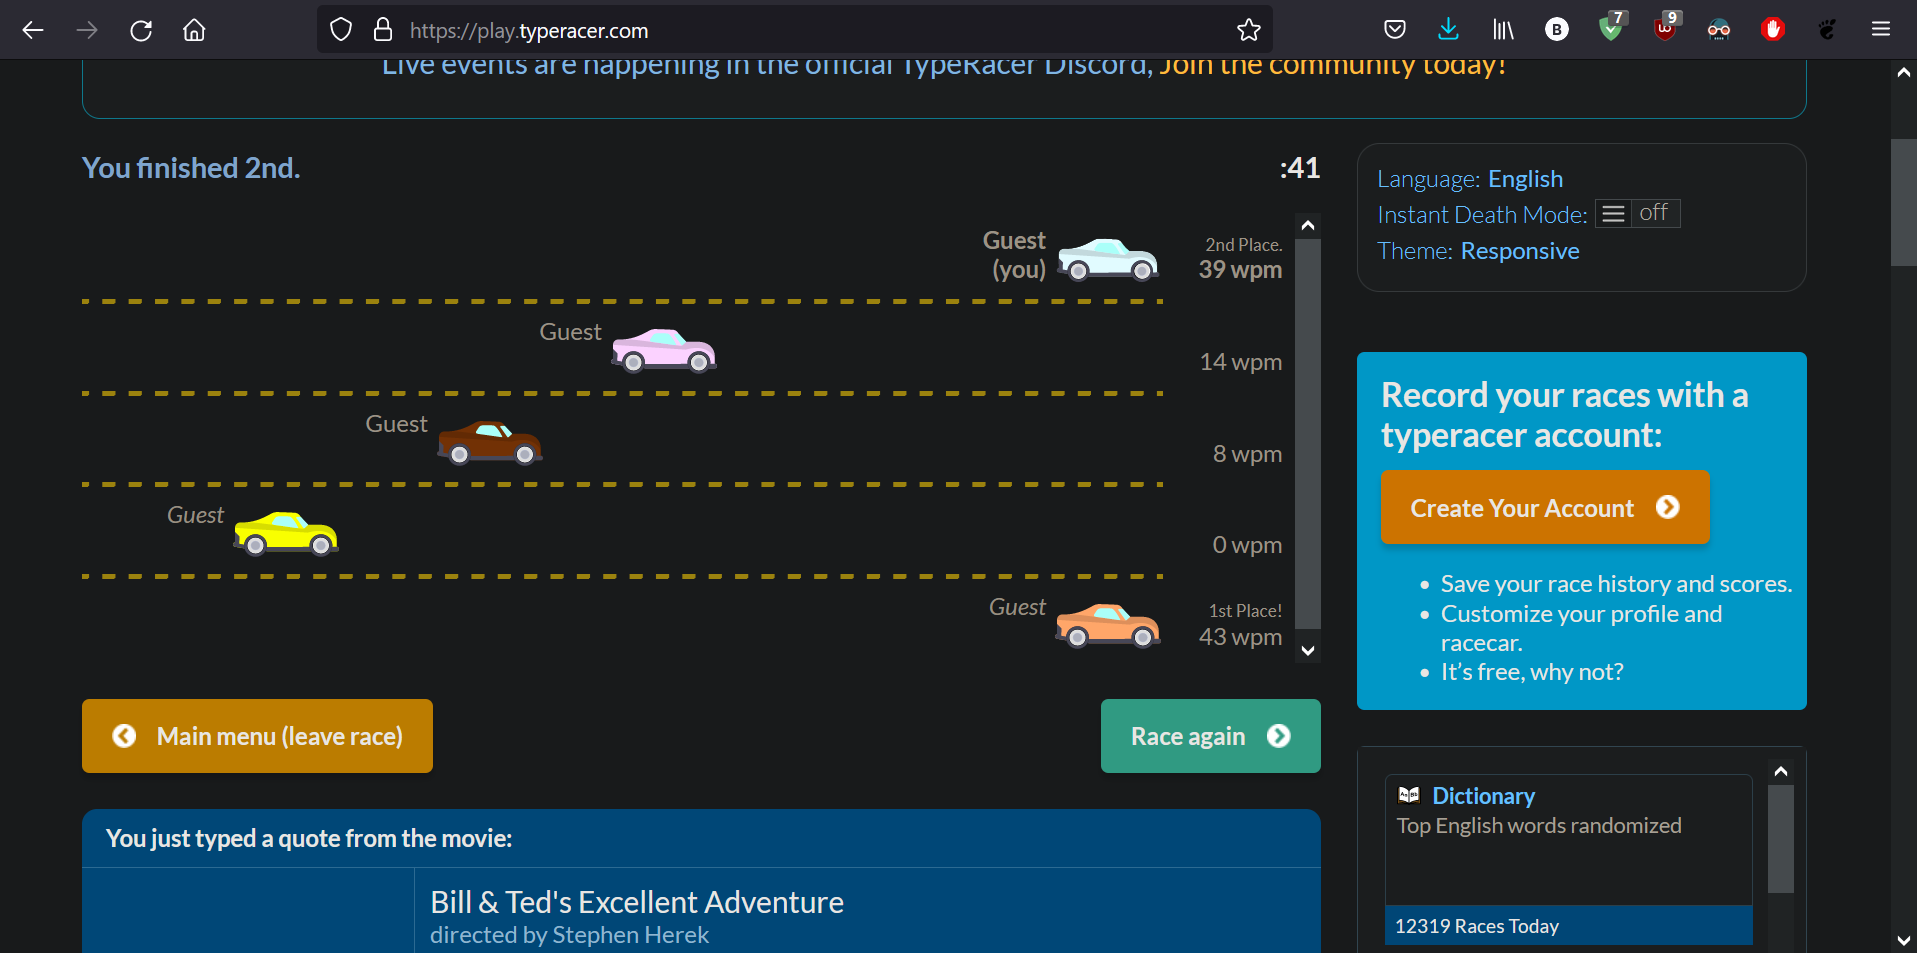
\includegraphics[scale=0.5]{image/typing.PNG}
\end{center}

\newpage

\subsection{Tutoriels Vim et Emacs} %2

\subsubsection*{Avec emacs}

\begin{enumerate}
\item Quitter emacs, ctrl + x puis ctrl + c
\item Descendre d'une page, ctrl + v
\item Monter d'une page, alt + v
\item Déplacer le cursor, ctrl + <Première lettre du mot de la direction> (Donc f pour forward b pour back etc...)
\end{enumerate}

Pour que emacs soit l'éditeur par défaut : update-alternatives --config editor

\subsection{History} %3

Pour supprimer des éléments de mon historique : export HISTIGNORE=ls ou cd ou pwd


\subsection{Alias} %5


\begin{commandline}
	\begin{verbatim}
function mkdcd () { mkdir "$1" && cd "$1" }
function gitemergency() {
	git add .
	git commit -a -m "$1"
	git push
	git status
}
	 \end{verbatim}
\end{commandline}

\subsection{Back up} %6
\noindent sudo update-alternatives --config editor \\

\begin{commandline}
	\begin{verbatim}
_backup() {
    local cur prev opts
    cur="${COMP_WORDS[COMP_CWORD]}"
    prev="${COMP_WORDS[COMP_CWORD-1]}"
    local files=("${cur}"*)
    case $COMP_CWORD in
        1) opts=`getent passwd | cut -d: -f1`;;
        2) opts="now tonight tomorrow";;
        3) opts="${files[@]}";;
        *);;
    esac
    COMPREPLY=()
    COMPREPLY=( $(compgen -W "$opts" -- ${cur}) )
    return 0
}
complete -o nospace -F _backup backup
	 \end{verbatim}
\end{commandline}

\subsection{ZSH Vagrant} %7

\begin{commandline}
	\begin{verbatim}
cd /home/arnaud/.oh-my-zsh/plugins/vagrant-prompt  
sudo nano vagrant-prompt.plugin.zsh
sudo nano ~/.zshrc
~/.oh-my-zsh/themes/robbyrussell.zsh-theme
	 \end{verbatim}
\end{commandline}
On ajoute dans ~/.oh-my-zsh/themes/robbyrussell.zsh-theme :

\begin{center}
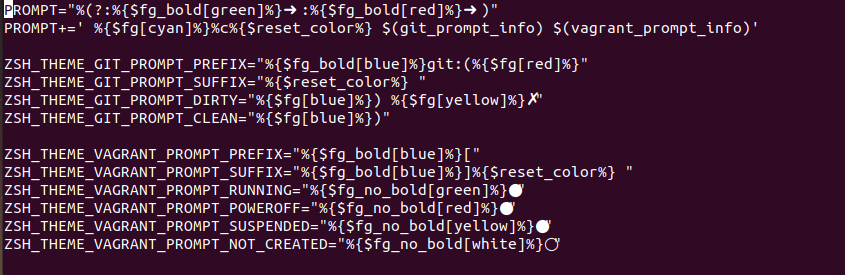
\includegraphics[]{image/zsh.png}
\end{center}

\subsection{Raccourci ZSH} %8
Dans le ~/.zshrc :

\begin{commandline}
	\begin{verbatim}
function apache_start() {
	if  /etc/init.d/apache2 status > /dev/null; then
        		echo "apache2 se stop"
	else
        		echo "le service apache2 est déja stoppé"
	fi
	sudo service apache2 stop
}

zle -N apache_start
bindkey "^b" apache_start

	\end{verbatim}
\end{commandline}

\newpage

\subsection{Emulateurs de terminaux}

\subsubsection{ Cool-Retro-Term}
\noindent Ce terminal simule un terminal old school avec un style Fallout.
Avec l’éditeur de texte « nano » il n’y a aucun code couleur avec ce terminal a part une typologie plus foncé lors des éléments importants.
Avec l’éditeur « Vim » la typologie des éléments importants est un peu plus rouge.
Ce terminal ne change pas grand-chose, c’est juste le style.

\begin{center}
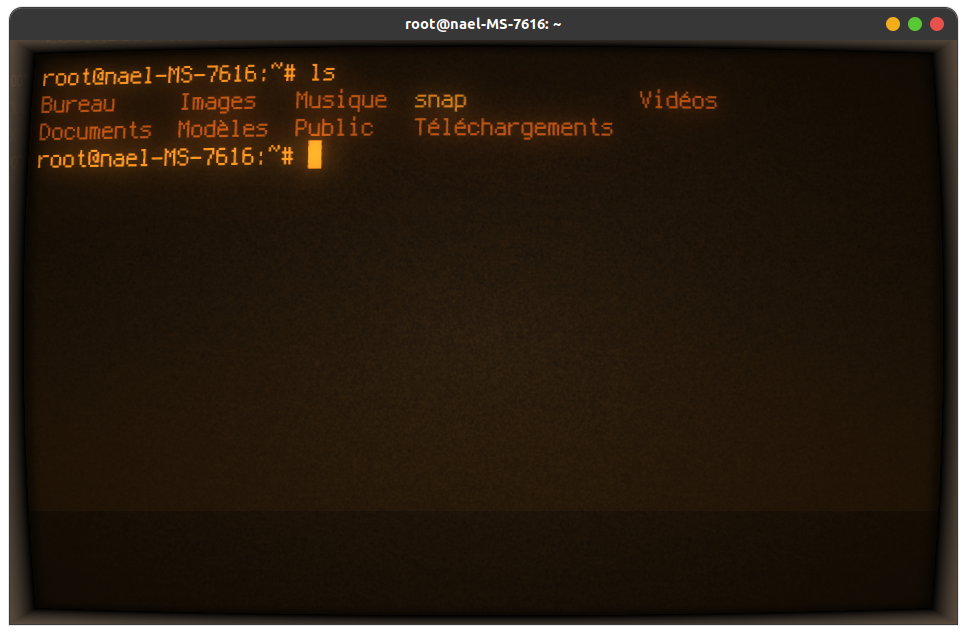
\includegraphics[scale=0.2]{image/coolRetroTerm.png}
\end{center}

\subsubsection{ eDEX-UI}
\noindent Fonctionnalités: Permet d'avoir plusieurs onglets en même temps, déplacement dans les dossiers depuis l'UI, informations sur l'utilisation de l'hardware, clavier virtuel pour écrans tactiles, différents thèmes pour différents goûts.

\noindent Rapidité: Assez rapide à lancer, mais réduit les performances

\begin{center}
\includegraphics[scale=0.2]{image/edexUI.png}
\end{center}

\subsubsection{ Terminator}
\noindent Terminal virtuel permettant une organisation plus simple des fenêtres car il permet d'avoir plusieurs terminaux dans une seule fenêtre.


\begin{center}
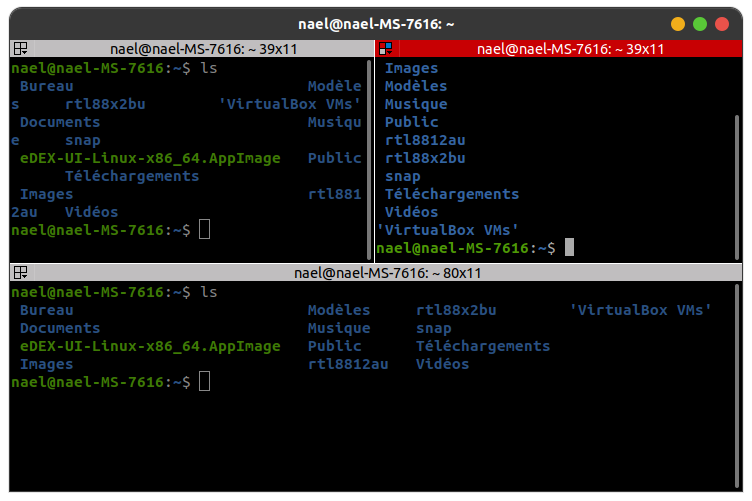
\includegraphics[scale=0.3]{image/terminator.png}
\end{center}

\section{(SSH)}

\subsection{Connection}
\noindent Ssh bob@10.0.0.2

On remarque que l'on n'a pas accès aux commandes lancées sur l'environnement Vagrant

\subsection{Clés privées et publiques} %9

\noindent ssh-keygen -b 4096 va ajouter une clé
\\
Pour ajouter la clée à l’utilisateur de la machine distante : ssh-copy-id alice@10.0.0.2
\\
Il nous faudra rentrer une passphrase pour la première connexion
\\
\\
Pour ajouter une clée publique manuellement sur notre machine hôte,  afficher notre clée plublique créé précédemment. Ensuite il faut se connecter à l'utilisateur de la machine souhaitée.
Il faut avoir un dossier .ssh ainsi qu'un fichier authorized\_keys dans le home de l'utilisateur. Ensuite, il faut copier la clée publique dans ce fichier.
\\
\\
Bonus :

\noindent Une passphrase est un "mot de passe" permettant de protéger une clée de cryptage
La clée de cryptage est dérivée de la passphrase pour chiffrer la ressource à protéger.
\\
\\
En exécutant ssh-add, cela va nous permettre de mettre notre passphrase en mémoire pour éviter de la taper a chaque connexion.

\subsection{Purge SSH} %10

\noindent Pour éviter de rentrer une empreinte lors de la première connexion :
il faut afficher l’empreinte de notre serveur sur le quel nous voulons nous connecter.
\\
\noindent ssh-keyscan -H 10.0.0.3

\noindent On l'ajoute dans notre /.ssh/known\_host. Cela nous permettra de nous connecter sans empreinte .
Il faut créer notre fichier config dans .ssh
\begin{commandline}
	\begin{verbatim}
Host bc # alias
Hostname 10.0.0.3 # ip machine
User bob # l’utilisateur au quel nous voulons nous connecter.
	\end{verbatim}
\end{commandline}

\noindent Après avoir exécuter ssh bc, nous serons directement connecté à bc avec l'utilisateur Bob.

\subsection{SFTP} %11

\noindent On se connecte en sftp à alice : sftp alice@10.0.0.2 
\\
\noindent get test \# pour prendre un fichier de la machine virtuelle vers notre machine.
\\
\noindent put test \# pour prendre un fichier de notre machine vers la machine vituelle.
\\
Pour synchroniser des répertoires de notre machine virtuelle à notre machine hôte avec sshfs.
\\
\noindent sshfs alice@10.0.0.2:/home /tmp/alicecli
\\
Le home de alice sera synchronisé et mis à jour dans notre répertoire /tmp/alicecli

\begin{warn}
Bien créer les répertoires avant, cette commande ne va pas les créer à votre place
\end{warn}

\noindent Si nous modifions notre fichier paratagée que ce soit sur notre machine hôte ou notre machine virtuelle les changements seront effectués dans les 2 sens.

\subsection{Tunnel SSH 1}

\noindent Depuis notre local host pour se connecter a notre serveur en passant par la vm CLI
\\
 ssh -L 8000:10.0.0.3:80 bob@10.0.0.2
\begin{warn}
10.0.0.3 est le serveur que nous voulons contacter et 10.0.0.2 est la machine par laquelle nous voulons passer pour se connecter au serveur
\end{warn}
une fois connecté a notre CLI il faut ouvrir un autre terminal et via notre machine host
\\
curl http://localhost:8000/cgi-bin/test1.cgi et nous aurons comme résultat :

\begin{center}
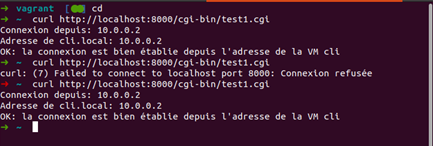
\includegraphics[]{image/curl.png}
\end{center}

Si nous coupons le tunnel sur bob@cli sur notre deuxième terminal le curl http://localhost:8000/cgi-bin/test1.cgi ne fonctionnera plus.

\subsection{Tunnel SSH 2}

\noindent ssh -L 9000:10.0.0.3:80 bob@10.0.0.2 
\\
Pour créer le tunnel, ensuite dans le terminal de notre machine hôte 
\\
ssh -D 9000 bob@cli.local 
\\
Pour créer le port 9000,

\noindent Installer tsocks.
\\
tsocks on
\\
tsocks firefox
\\
et dans l’url taper http://srv,local/test1…….etc
\\
et nous aurons accès à notre serveur via CLI .


\subsection{X11 Forwarding}

\noindent Sur le serveur on installe les paquets x server avec la commande : sudo apt install x11-apps
\\
En local sur notre machine on se connecte en ssh : ssh -X bob@10.0.0.2
\\
Quand nous sommes connectés sur le serveur nous pouvons exécuter une application graphique qui se lancera en local : 
\\
xeyes



\subsection{Rebonds}

\subsubsection{ProxyJump}

\noindent Il faut ajouter dans le fichier ~/.ssh/config

\begin{commandline}
	\begin{verbatim}
Host bastion
    Hostname 10.0.0.2
    User bob

Host srv
    Hostname 10.0.0.3
    ProxyJump bastion
    User bob
	\end{verbatim}
\end{commandline}
\noindent On se connecte avec ssh srv, en exécutant la commande who on voit l'adresse de CLI et non SRV

\subsubsection{ProxyCommand}

\begin{commandline}
	\begin{verbatim}
Host bastion
    Hostname 10.0.0.2
    User bob

Host srvcmd
    Hostname 10.0.0.3
    User bob
    ProxyCommand ssh bastion -W %h:%p
	\end{verbatim}
\end{commandline}

\noindent Cela revient au même avec ProxyCommand mais on laisse des traces sur le serveur passerelle.

\subsection{BONUS}

\section{Git}

\subsection{}
On crée un repository dans le répertoire : git init

On copie le vagrant file et dossier ssh dans le nouveau dossier

On les envoie sur le repository : git commit

On vérifie : git status

Les 2 fichiers apparaîtrons en rouge

On fait git add des 2 fichier

vagrant up

vagrant halt

On vérifie le repository : git status 

Nouveau ,vagrant/ apparaît en rouge
On créer le .gitignore dans le dossier

Ajouter le .vagrant 

lors d’un git status le vagrant ne s’affiche pas en rouge.

\subsection{}

On crée une nouvelle branche : git checkout -b branche

On ajoute l'utilisateur Patrick et on installe php et apache

On effectue les commit : git add -p Vagrantfile | git commit -m new "ajout du branche"

On revient sur la branche main : git checkout master

On vérifie que l'on n'a pas de modificationns : git log

Le working directory est comme on l'a laissé avant de créer la nouvelle branche

On fusionne les branches : git merge branche

On inspecte le commit : git log

On a bien les modifications

On vérifie si la branche existe toujours : git branch

Elle existe toujours mais on en a plus besoin

On supprime la branche : git branch -d branche

\subsection{}

On crée une nouvelle branche : git checkout -b forward-new-port

On modifie le VagrantFile et on commmit : git add Vagrant | git commmit -m "ajout du port"

On retourne sur main, on modifie le VagrantFile et on commit : git add Vagrant | git commmit -m "ajout du port"

On merge : git merge

On aura donc un conflit, il nous suffit de de modifier le fichier et de l'ajouter : git add VagrantFile

On vérifie que le conflit est résolu : git status

On termine le merge : git merge --continue 

\subsection{}


\end{document}

